\documentclass{article}
\usepackage{tikz}

\begin{document}

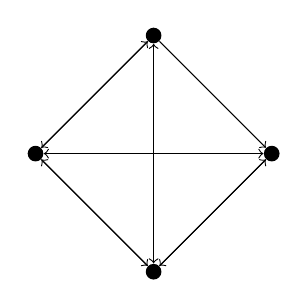
\begin{tikzpicture}[scale=1.5]
    % Define the nodes
    \node (A) at (0,0) [circle,fill,inner sep=2pt] {};
    \node (B) at (1,1) [circle,fill,inner sep=2pt] {};
    \node (C) at (2,0) [circle,fill,inner sep=2pt] {};
    \node (D) at (1,-1) [circle,fill,inner sep=2pt] {};
    
    % Draw the edges with arrows
    \draw[->] (A) -- (B);
    \draw[->] (A) -- (C);
    \draw[->] (A) -- (D);
    \draw[->] (B) -- (C);
    \draw[->] (B) -- (D);
    \draw[->] (C) -- (D);
    \draw[->] (B) -- (A);
    \draw[->] (C) -- (A);
    \draw[->] (D) -- (A);
    \draw[->] (D) -- (B);
    \draw[->] (D) -- (C);
\end{tikzpicture}

\end{document}